Przyjrzymy się więc jednej stronie powyższego dualizmu i przeanalizujmy kopuły jako struktury zależności.

\begin{df}[Kopuła minimum]
	Dwuwymiarowa kopuła minimum $C^{-}$ to kopuła zadana wzorem $C^{-}(u, v) = \max(u+v-1, 0).$
\end{df}
\begin{df}[Kopuła maximum]
	Dwuwymiarowa kopuła maksimum $C^{+}$, to kopuła zadana wzorem $C^{+}(u, v) = \min(u, v).$
\end{df}

\begin{figure}[h]
	\centering
	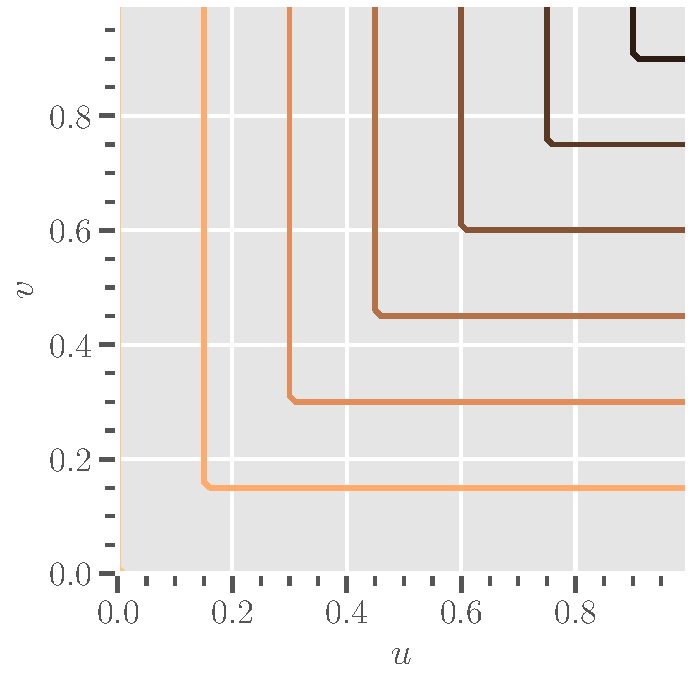
\includegraphics[width=0.35\linewidth]{01_MaximumCopula_contour}
	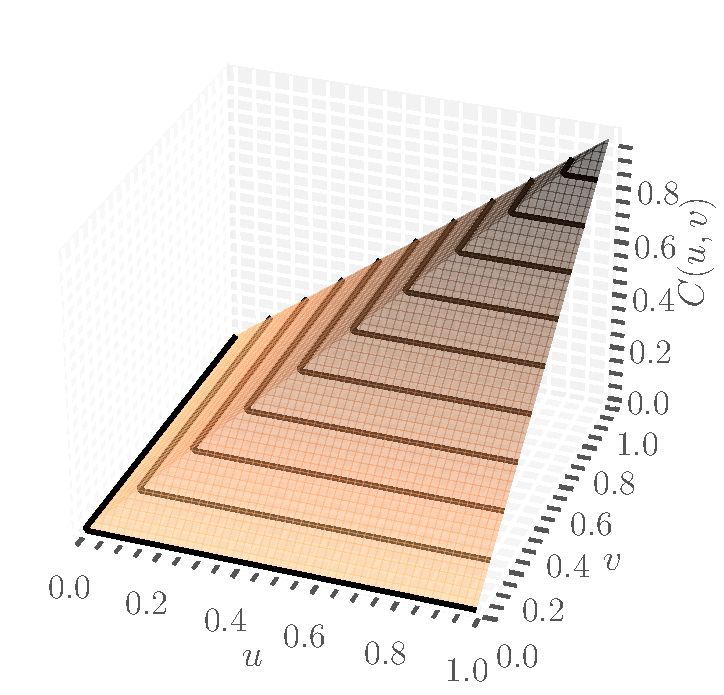
\includegraphics[width=0.4\linewidth]{01_MaximumCopula_surface}
	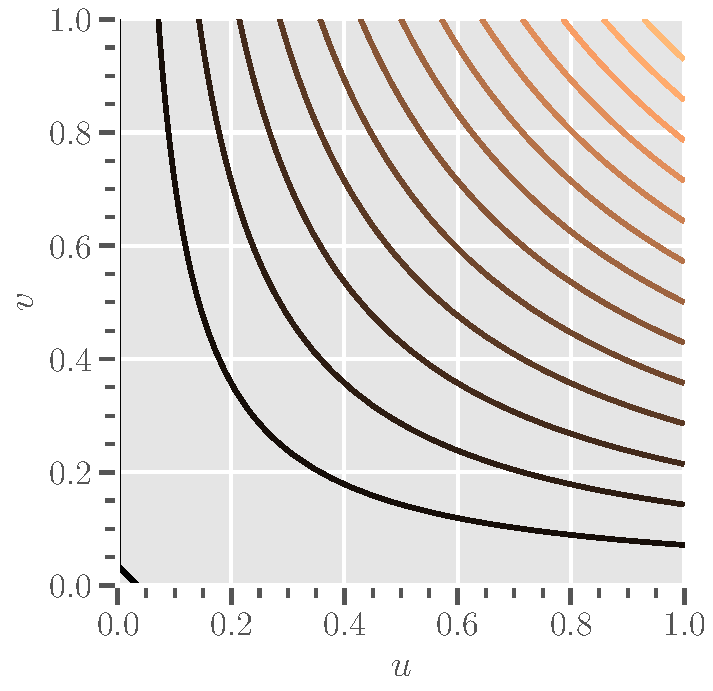
\includegraphics[width=0.35\linewidth]{01_IndependenceCopula_contour}
	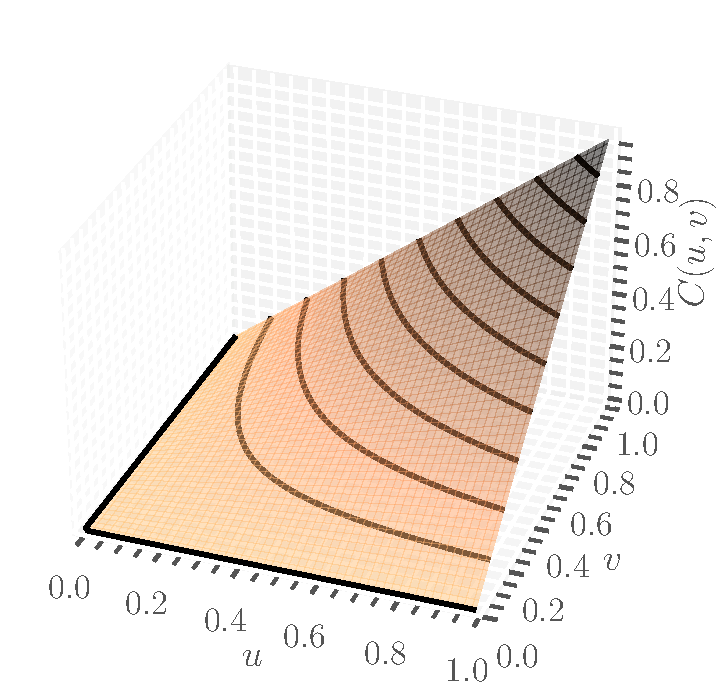
\includegraphics[width=0.4\linewidth]{01_IndependenceCopula_surface}
	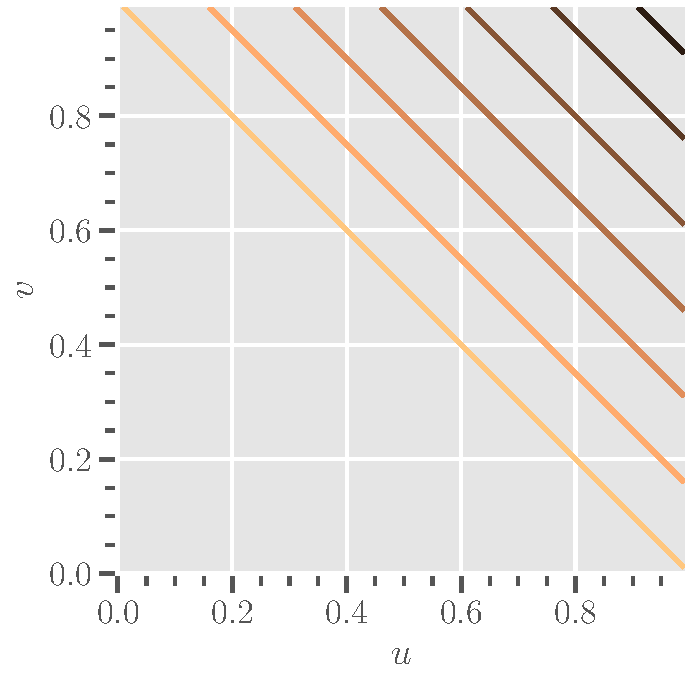
\includegraphics[width=0.35\linewidth]{01_MinimumCopula_contour}
	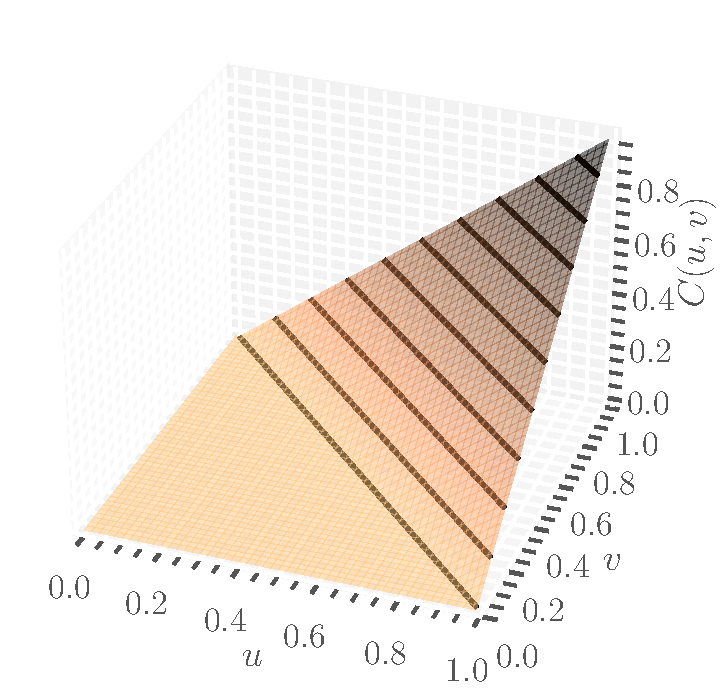
\includegraphics[width=0.4\linewidth]{01_MinimumCopula_surface}
	
	\caption{Dystrybuanty (po lewej) i kontury (po prawej) kopuł: maximum (górny panel), produktowej (panel środkowy) i minimum (dolny panel)\label{fig:minmaxprod_copula}}
\end{figure}

Powyższe kopuły stanowią horyzont osiągalnych kopuł, ponieważ jak mówi twierdzenie \ref{thm:frechet_hoeffding}, są one ograniczeniem dolnym i górnym dla dowolnej innej kopuli. Ich powierzchnie i kontury przedstawia rysunek \ref{fig:minmaxprod_copula}. 

\begin{thm}[Fréchet-Hoeffding bounds]
	Niech $C$ będzie $2$-wymiarową kopułą. Wtedy dla każdego $(u, v)\in[0, 1]^2$ zachodzi
	
	$$ C^{-}(u, v) \leqslant C(u, v) \leqslant C^{+}(u, v).$$
	
	\label{thm:frechet_hoeffding}
\end{thm}

Twierdzenie to, choć z pozoru teoretyczne, ciągnie za sobą bardzo praktyczne konsekwencje: pozwala otrzymać niezależne od modelu ogranicznia górne i dolne na dowolną kopułę. \cite{Cherubini_Copula_Methods_in_Finance} pokazuje przykład, gdzie twierdzenie Frécheta-Hoeffdinga pozwala na uzyskanie dolnego i górnego ograniczenia na pewne statystyki modelu, jak np. łączne prawdopodobieństwo bankructwa dwóch firm w strukturalnym modelu Mertona, czy cena opcji binarnej na dwa aktywa.

\begin{df}[Kopuła produktowa]
	Dwuwymiarowa kopuła produktowa $C^{\perp}$ to kopuła zadana wzorem $C^{\perp}(u, v) = uv.$
\end{df}

Kopuła produktowa jest trzecim istotnym punktem odniesienia w świecie kopuł, ponieważ posiada pewną unikalną właśność. Z jednej strony z definicji kopuły mamy:

\begin{equation}
C(u, v) = P(U \leqslant u, V \leqslant v )
\label{eq:independence_copula1}
\end{equation}

Z drugiej jednak strony, wiemy że $U$ i $V$ mają rozkłady jednostajne - więc:
\begin{equation}
	F_U(u) = P(U \leqslant u) = u\text{, oraz } F_V(v) = P(V \leqslant v) = v.
\label{eq:independence_copula2}
\end{equation}

Z równań \ref{eq:independence_copula1} i \ref{eq:independence_copula2}, dla przypadku kopuły produktowej mamy zatem:
\begin{equation}
	P(U \leqslant u, V \leqslant v ) \equiv C^{\perp}(u, v) = uv = P(U \leqslant u) P(V \leqslant v).
	\label{eq:independence_copula}
\end{equation}

Równanie \ref{eq:independence_copula} mówi nam, że zmienne losowe $V$ i $U$ są od siebie niezależne. Model kopuły produktowej, implikuje więc niezależność jednostajnych rozkładów brzegowych.
Co więcej, uzupełniając opis kopuł minimum i maksimum - te z kolei odpowiadają współmonotonicznej \emph{(eng. comonotone)} i przeciwmonotonicznej \emph{(eng. countermonotone)} zależności jednostajnych rozkładów brzegowych. Zgodnie z twierdzeniem \ref{thm:frechet_hoeffding} natomiast wszystkie inne kopuły modelują pozostałe rodzaje zależności istniejące pomiędzy tymi ekstremami. Widzimy więc, że kopuły potrafią modelować pełne spektrum możliwych zależności: od współmonotonicznych, przez niezależne, aż po przeciwmonotoniczne. 